\documentclass[11pt,letterpaper]{article}

\usepackage[T1]{fontenc}
\usepackage{lmodern}
\usepackage{textcomp}
\usepackage[margin=1in]{geometry}
\usepackage{amsmath,amssymb}
\usepackage{graphicx}
\usepackage{booktabs}
\usepackage{tabularx}
\usepackage{microtype}
\usepackage{xcolor}
\usepackage{hyperref}

\makeatletter
\g@addto@macro\UrlBreaks{\do\/\do\-\do\_\do\.\do\a\do\b\do\c\do\d\do\e\do\f\do\g\do\h\do\i\do\j\do\k\do\l\do\m\do\n\do\o\do\p\do\q\do\r\do\s\do\t\do\u\do\v\do\w\do\x\do\y\do\z}
\makeatother

\hypersetup{
    colorlinks=true,
    linkcolor=blue!80!black,
    citecolor=blue!80!black,
    urlcolor=blue!80!black
}

\title{\textbf{Verifiable Agentic Science on Public Infrastructure}}

\author{
  Dannon Baker$^{1}$, Marius van den Beek$^{2}$, John Chilton$^{2}$,\\
  Danielle Callan$^{2}$, Scott Cain$^{2}$, Steven Weaver$^{3}$,\\
  Sergei L. Kosakovsky Pond$^{3,*}$, and Anton Nekrutenko$^{2,*}$\\[0.8em]
  \small $^{1}$Department of Biology, Johns Hopkins University, Baltimore, MD, USA\\
  \small $^{2}$Department of Biochemistry and Molecular Biology, Penn State University, University Park, PA, USA\\
  \small $^{3}$Institute for Genomics and Evolutionary Medicine, Department of Biology,\\
  \small Temple University, Philadelphia, PA, USA\\[0.3em]
  \small $^{*}$Correspondence: \texttt{spond@temple.edu}, \texttt{anton@nekrut.org}
}

\date{\today}

\begin{document}

\maketitle

\begin{abstract}
Frontier artificial intelligence models promise to accelerate scientific discovery by automating hypothesis formulation, experimental design, and computational code execution across complex biological domains. Yet contemporary agent platforms operate as disembodied reasoning engines in isolated local environments, generating unversioned scripts, overwhelming consumer hardware on large datasets, and confining scientific discovery to proprietary corporate enclosures. We eliminate this computational bottleneck. Here we introduce an open agentic architecture that provides artificial intelligence with a distributed computational body, transforming public Galaxy cyberinfrastructure into an execution surface governed by immutable directed acyclic graph provenance. To direct long-horizon investigations, we develop Orbit, a scientific research workbench that binds human intent, execution decisions, and remote cloud invocations into a version-controlled research notebook. Complementing this workbench, the Workflow Foundry compiles scientific literature into schema-validated workflows, while unprivileged User-Defined Tools allow agents to execute containerized commands across public supercomputing clusters without administrative intervention. By establishing provenance by construction, this infrastructure prevents the hallucination of scientific method, resolving silent gene identifier traps and converting external workflows into reproducible community assets. All software and universal plugins are freely available, ensuring verifiable scientific discovery across the open public commons.
\end{abstract}

\section{Introduction}

Scientific inquiry faces a profound epistemological crisis. The rapid emergence of autonomous artificial intelligence agents promises to compress years of computational investigation into hours, allowing language models to formulate hypotheses, select algorithms, and author code across diverse domains of life science \cite{biocoder2024}. Yet without rigorous computational grounding, this acceleration threatens the foundation of scientific truth. Left unconstrained, frontier models generate persuasive but unobservable computational fiction---a phenomenon we define as the hallucination of method. Agents author bespoke scripts in transient directories, omit software dependency versions, and manipulate raw data through unrecorded ad hoc transformations. The resulting analyses appear mathematically rigorous and biologically sound, yet rest upon ephemeral code fragments that defy replication. In computational biology, where conclusions depend entirely on software parameterization and execution lineage, unrecorded agency produces post-verifiable science. 

The root of this crisis lies in a fundamental structural misspecification: the mind-body problem of artificial intelligence. For the past three years, automated scientific platforms have operated as disembodied reasoning engines. Systems celebrate the ability of foundation models to debate hypotheses, synthesize literature, or write short script sequences within isolated local sandboxes. Yet empirical science cannot occur in a vacuum. A disembodied reasoning engine cannot interact with petabytes of raw sequence archives, cannot schedule jobs across distributed high-performance clusters, and cannot allocate multi-node physical memory. Operating on personal computers, autonomous agents quickly collide with physical reality. Workstations run out of memory during genome assembly, crash under high-throughput read alignment, or silently truncate input files to fit within local constraints. A mind without a computational body is an armchair philosopher, incapable of executing authentic empirical investigations.

This computational limitation exacerbates a dangerous institutional shift: the privatization of scientific discovery. As frontier foundation models demand vast computational resources, high-capability scientific automation is increasingly sequestered inside commercial walled gardens. Proprietary corporate research platforms link foundation models to private compute clusters and closed cloud storage. This enclosure creates an unequal scientific world. Well-funded commercial institutions conduct automated research at scale, while academic laboratories and researchers in resource-limited environments remain stranded on personal workstations. Commercial platforms occasionally provide static session transcripts or rendered cards, but these artifacts offer only the illusion of reproducibility. An independent researcher cannot re-execute a proprietary conversational transcript, cannot inspect its container layers, and cannot run the underlying code on independent infrastructure. Science risks trading open, universal verification for private corporate authority.

Recent automated research platforms illustrate these architectural trade-offs. The AI Scientist demonstrated fully automated machine learning discovery, generating hypotheses, executing code, and authoring complete manuscripts \cite{aiscientist2024}. However, its execution was restricted to toy algorithmic scripts inside isolated local directories, where unconstrained execution led to hallucinated citations, runaway loops, and unverified numerical claims. Automated discovery stalled on computational rigor. Google DeepMind recently introduced Co-Scientist, a multi-agent framework that implements structured debate to generate and evolve biomedical research proposals \cite{coscientist2026}. While Co-Scientist produced validated therapeutic hypotheses for drug repurposing, the system acts primarily as a literature reasoning engine, yielding descriptive textual plans rather than executable, cloud-backed computational workflows that can process terabyte-scale biological data. The Virtual Lab demonstrated comparable trade-offs \cite{virtuallab2025}. Coordinating specialized agent personas---principal investigators, scientific critics, and bioinformaticians---the platform designed viable SARS-CoV-2 nanobodies with laboratory validation, yet its computational execution relied on bespoke local scripts that lacked a standardized, shareable execution graph. Kosmos addressed session persistence by employing a structured world model across twelve-hour investigations \cite{kosmos2025}. Nevertheless, its computational runtime remains confined to basic sandboxes that cannot orchestrate multi-node compute schedules or petabyte-scale public archives.

Domain tool orchestration faces identical structural boundaries. Platforms such as Coscientist \cite{boiko2023} and ChemCrow \cite{chemcrow2024} established that large language models can orchestrate specialized chemical synthesis hardware, external computational APIs, and safety protocols. They proved the power of tool augmentation. However, these systems were tailored specifically to small-molecule chemistry and laboratory robotics. They do not address the complex data structures of computational genomics---including paired-end sequencing collections, multi-sample variant calls, and distributed pipeline dependencies---across heterogeneous academic and commercial clusters. In parallel, commercial developer environments provide rapid software engineering capabilities on local files. Yet these platforms remain blind to biological context. While commercial code assistants parse syntax swiftly, they possess no native knowledge of reference genomes, biological format specifications, or high-performance compute allocations across supercomputing clusters. The investigator remains stranded on an isolated laptop with unpinned dependencies and fragmented scripts. Science requires a shared execution fabric.

Public scientific cyberinfrastructure provides the foundation to resolve these dilemmas. For two decades, the Galaxy platform has maintained an open, community-governed computational ecosystem designed to execute distributed scientific workflows across heterogeneous supercomputing clusters \cite{galaxy2024}. In the agentic era, Galaxy's graphical web interface becomes secondary. The platform instead emerges as an infrastructural agentic surface. Through standardized programmatic interfaces, Galaxy provides autonomous agents with immediate access to thousands of containerized bioinformatics tools, petabyte-scale reference data tables, and national high-performance compute allocations without requiring administrative intervention for every user command. Immutable directed acyclic graphs track every input dataset, exact tool revision, execution parameter, and intermediate file. Provenance is preserved by construction rather than through retroactive human discipline.

Here we present an open agentic architecture that bridges autonomous reasoning directly to distributed public computing infrastructure. The framework unites four computational components. First, we introduce Orbit, an open-source scientific research workbench that records hypotheses, analytical plans, execution logs, and cloud invocations directly into a living, version-controlled research notebook. Second, we develop the Workflow Foundry, a casting compiler that translates external scientific literature, Nextflow pipelines \cite{nextflow2017}, and Common Workflow Language specifications \cite{cwl2022} into schema-validated Galaxy workflows, eliminating language model hallucination through deterministic graph validation. Third, we establish User-Defined Tools, unprivileged containerized definitions that allow agents to register and run custom tools on remote Galaxy compute clusters safely using sandboxed ECMAScript templating. Fourth, we provide production plugins across major agent platforms---including Claude Code, Google Antigravity, and OpenAI Codex---allowing investigators to connect frontier models to public cyberinfrastructure. By grounding autonomous agents in public infrastructure, we replace isolated computational silos with verifiable, reproducible scientific discovery.

\section{The Flow: Agent \texorpdfstring{$\to$}{->} Infrastructure \texorpdfstring{$\to$}{->} Result}

Empirical biological discovery follows a structured journey: from experimental hypothesis to verified computational result. Our architecture implements this journey as a transparent three-stage pipeline (Figure~\ref{fig:architecture}). Investigators can use any autonomous agent runtime, including our custom workbench, Orbit, designed specifically with life scientists in mind. These agents draw domain knowledge directly from the Galaxy Model Context Protocol (MCP), curated Galaxy skills, and Workflow Foundry casting rules. Depending on local hardware availability, the agent prototypes and tests analytical logic on subsampled data before launching full-scale execution across Galaxy cyberinfrastructure. All analytical steps record into an immutable research notebook. This record establishes complete provenance by construction.

\begin{figure*}[htbp]
\centering
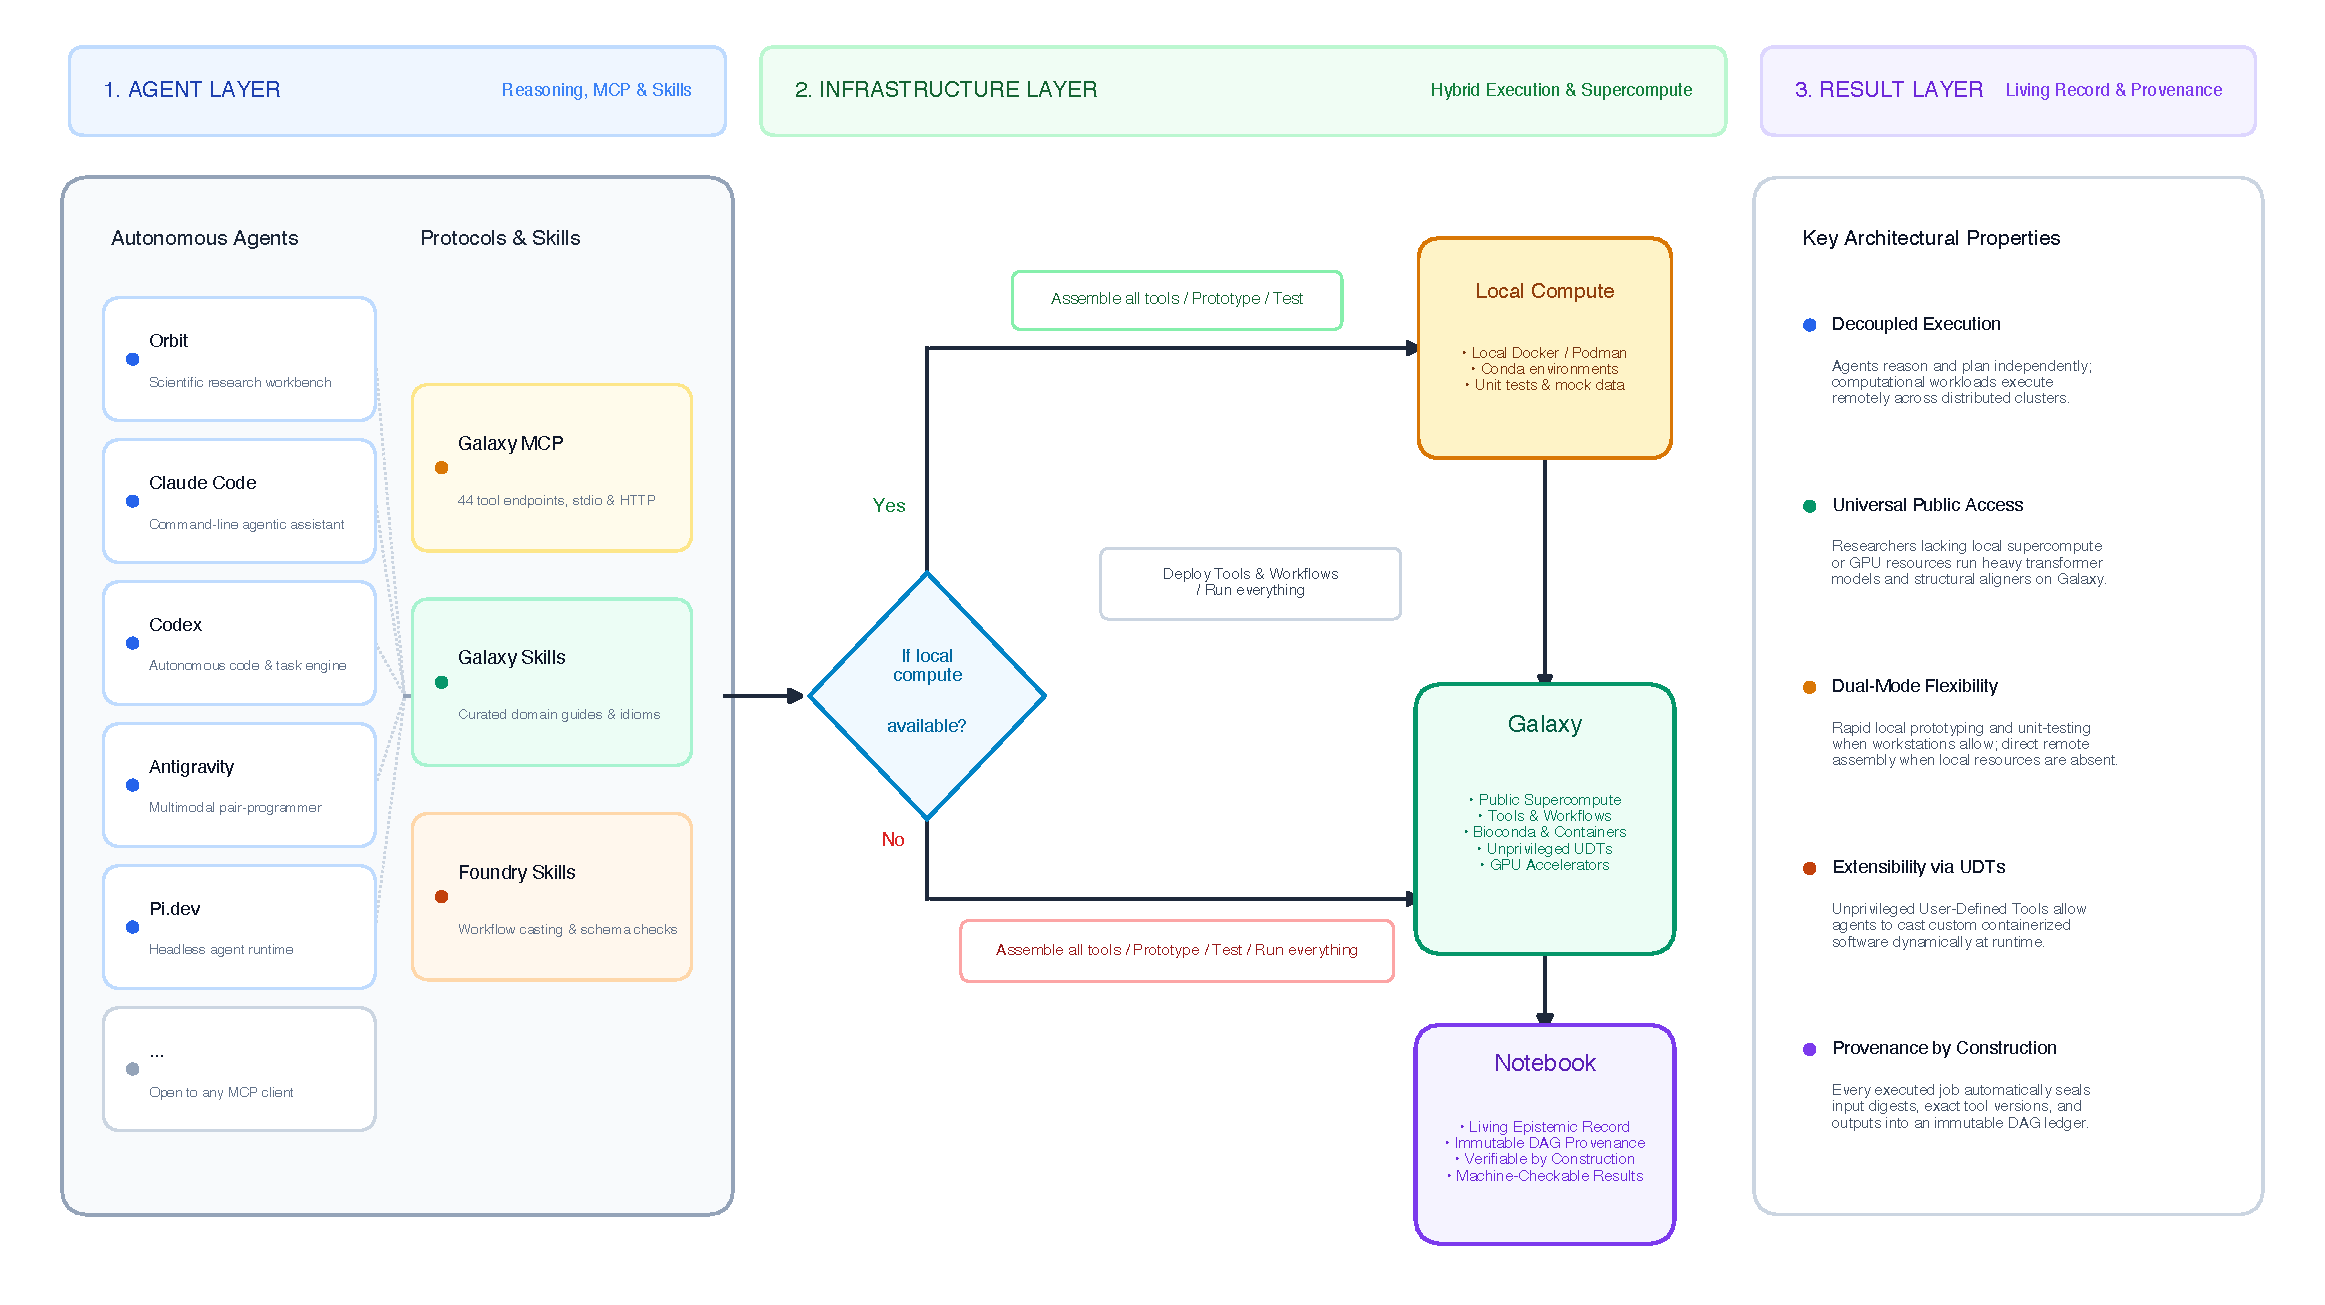
\includegraphics[width=\textwidth]{figures/figure1_architecture.pdf}
\caption{\textbf{The flow of verifiable agentic science: from Agent through Infrastructure to Result.} Autonomous agents---including Orbit, Claude Code, OpenAI Codex, Google Antigravity, and Pi.dev---interact with computational services via the Galaxy Model Context Protocol (MCP), Galaxy skills, and Foundry skills (Agent Layer). Execution branches based on local computational capacity. When local compute is available, agents assemble tools, prototype logic, and run unit tests locally before launching jobs and workflows on Galaxy. When local compute is absent, agents assemble, prototype, test, and execute the complete analytical workflow directly on Galaxy public cyberinfrastructure (Infrastructure Layer). Galaxy executes tasks across distributed supercomputing allocations and GPU clusters via native tools, BioContainers, and unprivileged User-Defined Tools. All analytical operations record directly into a living research notebook. This record preserves an immutable directed acyclic graph with machine-checkable results (Result Layer).}
\label{fig:architecture}
\end{figure*}

\subsection{Agents and the Orbit Workbench}
The architecture is completely agent-agnostic. Researchers are not tied to a single artificial intelligence vendor or proprietary chat interface. Instead, Galaxy can be driven directly by any compliant agent runtime. To facilitate adoption, we distribute open-source plugin packages for leading agent ecosystems, including Claude Code, OpenAI Codex, Google Antigravity, Cursor, and the Pi runtime \cite{agenticplugins2026}. Investigators retain their preferred development environment while connecting directly to public supercomputing resources.

To support biologists directly, we developed Orbit \cite{orbit2026}. General-purpose coding assistants assume deep familiarity with command-line interfaces, POSIX shell idiosyncrasies, and cloud environments. In contrast, Orbit provides a dedicated research environment that unifies conversational planning, interactive data visualization, and remote compute orchestration.

Orbit operates flexibly across model providers. Investigators can connect commercial frontier models, including Anthropic Claude, OpenAI GPT, or Google Gemini. Alternatively, researchers handling sensitive clinical data can run private local models through Ollama without transmitting data to external commercial APIs. Orbit incorporates built-in convenience features tailored for life scientists. The workbench manages Galaxy server credentials, polls running cloud jobs asynchronously in the background, renders intermediate datasets, and presents proposed analytical plans for human review before execution begins.

\subsection{The Galaxy Model Context Protocol and Skills}
Agents interact with computational infrastructure through the Galaxy Model Context Protocol server \cite{galaxymcp2026}. The Model Context Protocol establishes an open standard for tool execution and data inspection. Rather than allowing agents to execute arbitrary local shell commands, the server provides forty-four structured endpoints. These endpoints enable agents to search tool registries, inspect dataset collections, launch workflows, and monitor execution states through standard input-output streams or remote HTTP connections.

Domain expertise is provided through modular skill packages \cite{galaxyskills2026}. These skills teach language models standard bioinformatics conventions. Skills guide tool discovery, parameter selection, and collection manipulation idioms. For complex multi-step pipelines, Workflow Foundry skills compile validated workflow templates directly into agent memory \cite{foundry2026}. By separating operational skills from the underlying compute runtime, the framework ensures that agents execute verified analytical procedures rather than generating unvalidated guesses.

\subsection{Local Prototyping and Verification}
When local compute resources are available, agents adopt a disciplined, iterative prototyping workflow (Figure~\ref{fig:architecture}). On Unix-based operating systems such as macOS and Linux, workstations typically possess container runtimes and native POSIX shells. In contrast, Windows environments often encounter operational friction. Windows systems frequently lack native POSIX environments, suffer line-ending incompatibilities, or restrict container execution when virtualization features are unconfigured. When local resources are available, the agent proceeds through six sequential steps:

\begin{enumerate}
    \item \textbf{Formulate an analytical plan.} The agent outlines the biological objectives, required data transformations, and statistical tests.
    \item \textbf{Obtain human approval.} The investigator reviews the drafted plan, inspects proposed assumptions, and grants explicit permission to proceed.
    \item \textbf{Identify software dependencies.} The agent determines which computational tools, libraries, and container images are required.
    \item \textbf{Prototype on subsampled data.} The agent extracts a representative subset of reads or sequences to test the analytical logic rapidly.
    \item \textbf{Verify execution integrity.} The agent confirms that commands exit successfully, output files match expected schemas, and quantitative metrics appear biologically sensible.
    \item \textbf{Map tools to the Galaxy catalog.} The agent surveys the target Galaxy instance to identify which tools are pre-installed in the Tool Shed and which components must be provisioned as User-Defined Tools.
\end{enumerate}

This prototyping loop catches algorithmic flaws early. Testing on small datasets avoids wasting expensive supercomputer allocations on defective scripts.

\subsection{Distributed Remote Compute on Galaxy Cyberinfrastructure}
Once verified on local data, full-scale analyses transition to Galaxy cyberinfrastructure \cite{galaxy2024}. Modern Galaxy instances provide immense computational power. Public servers maintain thousands of community-curated, peer-reviewed tools spanning every domain of computational biology. Compute jobs route transparently to national supercomputing centers, high-performance clusters, and specialized hardware accelerators without requiring researchers to manage cluster schedulers. Furthermore, Galaxy maintains petabyte-scale reference data collections, eliminating the need to download large genome indices to local machines.

This infrastructure eliminates a pervasive pathology of autonomous coding agents. Standard agents routinely generate ad hoc Python scripts, store unversioned code in obscure subdirectories, and dump intermediate files into transient temporary directories. Once the agent terminates, nobody knows which code executed, which dependencies were active, or where intermediate data reside. Reproducibility becomes impossible.

Galaxy solves this problem through immutable histories. Every tool execution, exact parameter value, container digest, and intermediate dataset is recorded directly within a persistent directed acyclic graph. Biologists can inspect raw command lines, evaluate standard output logs, view graphical visualizations, and verify every analytical step. However, real-world biological workflows inevitably require custom utilities. Standard tool registries cannot anticipate every bespoke file format converter or novel software utility. For these missing glue steps, the architecture relies on User-Defined Tools.

\subsection{Extensibility via User-Defined Tools}
User-Defined Tools (UDTs) provide dynamic extensibility on public infrastructure \cite{galaxyudt2026}. Introduced in Galaxy 26.1, UDTs allow unprivileged users and autonomous agents to register and run custom tools dynamically. A UDT is declared as a compact YAML specification that pairs an immutable container image with typed inputs and an isolated command template. Because templates evaluate using sandboxed ECMAScript rather than arbitrary host scripts, custom tools execute safely on shared supercomputing clusters.

UDTs span a broad spectrum of computational complexity. At one end, an agent can author a lightweight UDT in seconds to convert unusual tabular formats, filter metadata, or glue disparate workflow steps together. At the opposite end, UDTs orchestrate heavy foundation models requiring dedicated GPU acceleration. Later in this manuscript, we demonstrate this capability in our \textit{Plasmodium vivax} case study. There, the agent authors custom UDTs that route 4.4-gigabyte protein language models directly to NVIDIA A100 GPUs on national supercomputers, executing complex structural alignments without manual system administration.

\subsection{Living Research Notebooks and Shared Provenance}
Every completed analysis yields two complementary artifacts: an executable Galaxy history and a living research notebook. While the Galaxy history preserves the physical data lineage, the research notebook captures the epistemic narrative. Structured similarly to an \texttt{AGENTS.md} record, the notebook documents the complete scientific context: initial hypotheses, biological motivations, human review checkpoints, and quantitative interpretations.

This pairing establishes complete computational provenance. Rather than receiving an isolated PDF report with static figures, independent researchers receive the entire experimental fabric. Galaxy histories, living notebooks, and containerized tool definitions can be published, cited, and shared via persistent URLs. Collaborators can inspect every intermediate dataset, examine why specific parameters were chosen, or re-execute the complete pipeline on public computing resources with a single click. By coupling autonomous agents to open infrastructure, biological discovery becomes fully transparent, verifiable, and reproducible.

\section{Empirical Results and Case Studies}

To evaluate the operational performance, reproducibility, and computational integrity of this architecture, we conduct three real-world scientific investigations spanning ad hoc empirical reanalysis, literature extraction, and cross-ecosystem pipeline conversion.

\subsection{Case Study 1: Heavy-Weight Model Orchestration and Structure-Aware Phylogenomics}

Empirical biological discovery frequently requires specialized analytical operations that exceed the boundaries of pre-installed tool registries. Standard agent benchmarks evaluate toy script generation on synthetic problems. In contrast, real-world biological workflows demand complex deep-learning foundational models, structural aligners, and dedicated hardware acceleration. We evaluated our agentic architecture on the structure-aware phylogenomics of the \textit{Plasmodium vivax} PIR multigene family (termed \textit{vir} in \textit{P. vivax}). Operating across three continental reference assemblies, the agent conducted the complete investigation on public cyberinfrastructure (UseGalaxy.org History \texttt{bbd44e69cb8906b579031c61c5da0079}).

\subsubsection*{Objective and Biological Rationale}
The PIR superfamily represents the largest multigene family in the \textit{Plasmodium vivax} genome. VIR surface antigens govern immune evasion, cytoadherence, and red blood cell rosetting (Fig.~\ref{fig:pathogenesis_rosetting}). Because PIR proteins undergo rapid sequence diversification, conventional sequence-based clustering over-splits the family into dozens of artificial subfamilies. Yet crystallographic structures reveal that PIR proteins share a single conserved, mostly-$\alpha$-helical fold (PDB 6ZYV, Fig.~\ref{fig:pathogenesis_rosetting}e). Sequence-based homology fails within this structural twilight zone.

We sought to determine whether structure-aware phylogenomics unifies the \textit{vir} repertoire across geographically distant isolates. We analyzed three chromosomal long-read reference assemblies: PvP01 from Indonesia, PvW1 from Thailand, and PvPAM from Peru. The study addressed two fundamental questions. First, does structural clustering collapse over-split sequence subfamilies into unified structural classes? Second, does the antigenic repertoire carry geographic lineage structure across continents, or does structural diversity predate continental radiation?

\begin{figure*}[htbp]
\centering
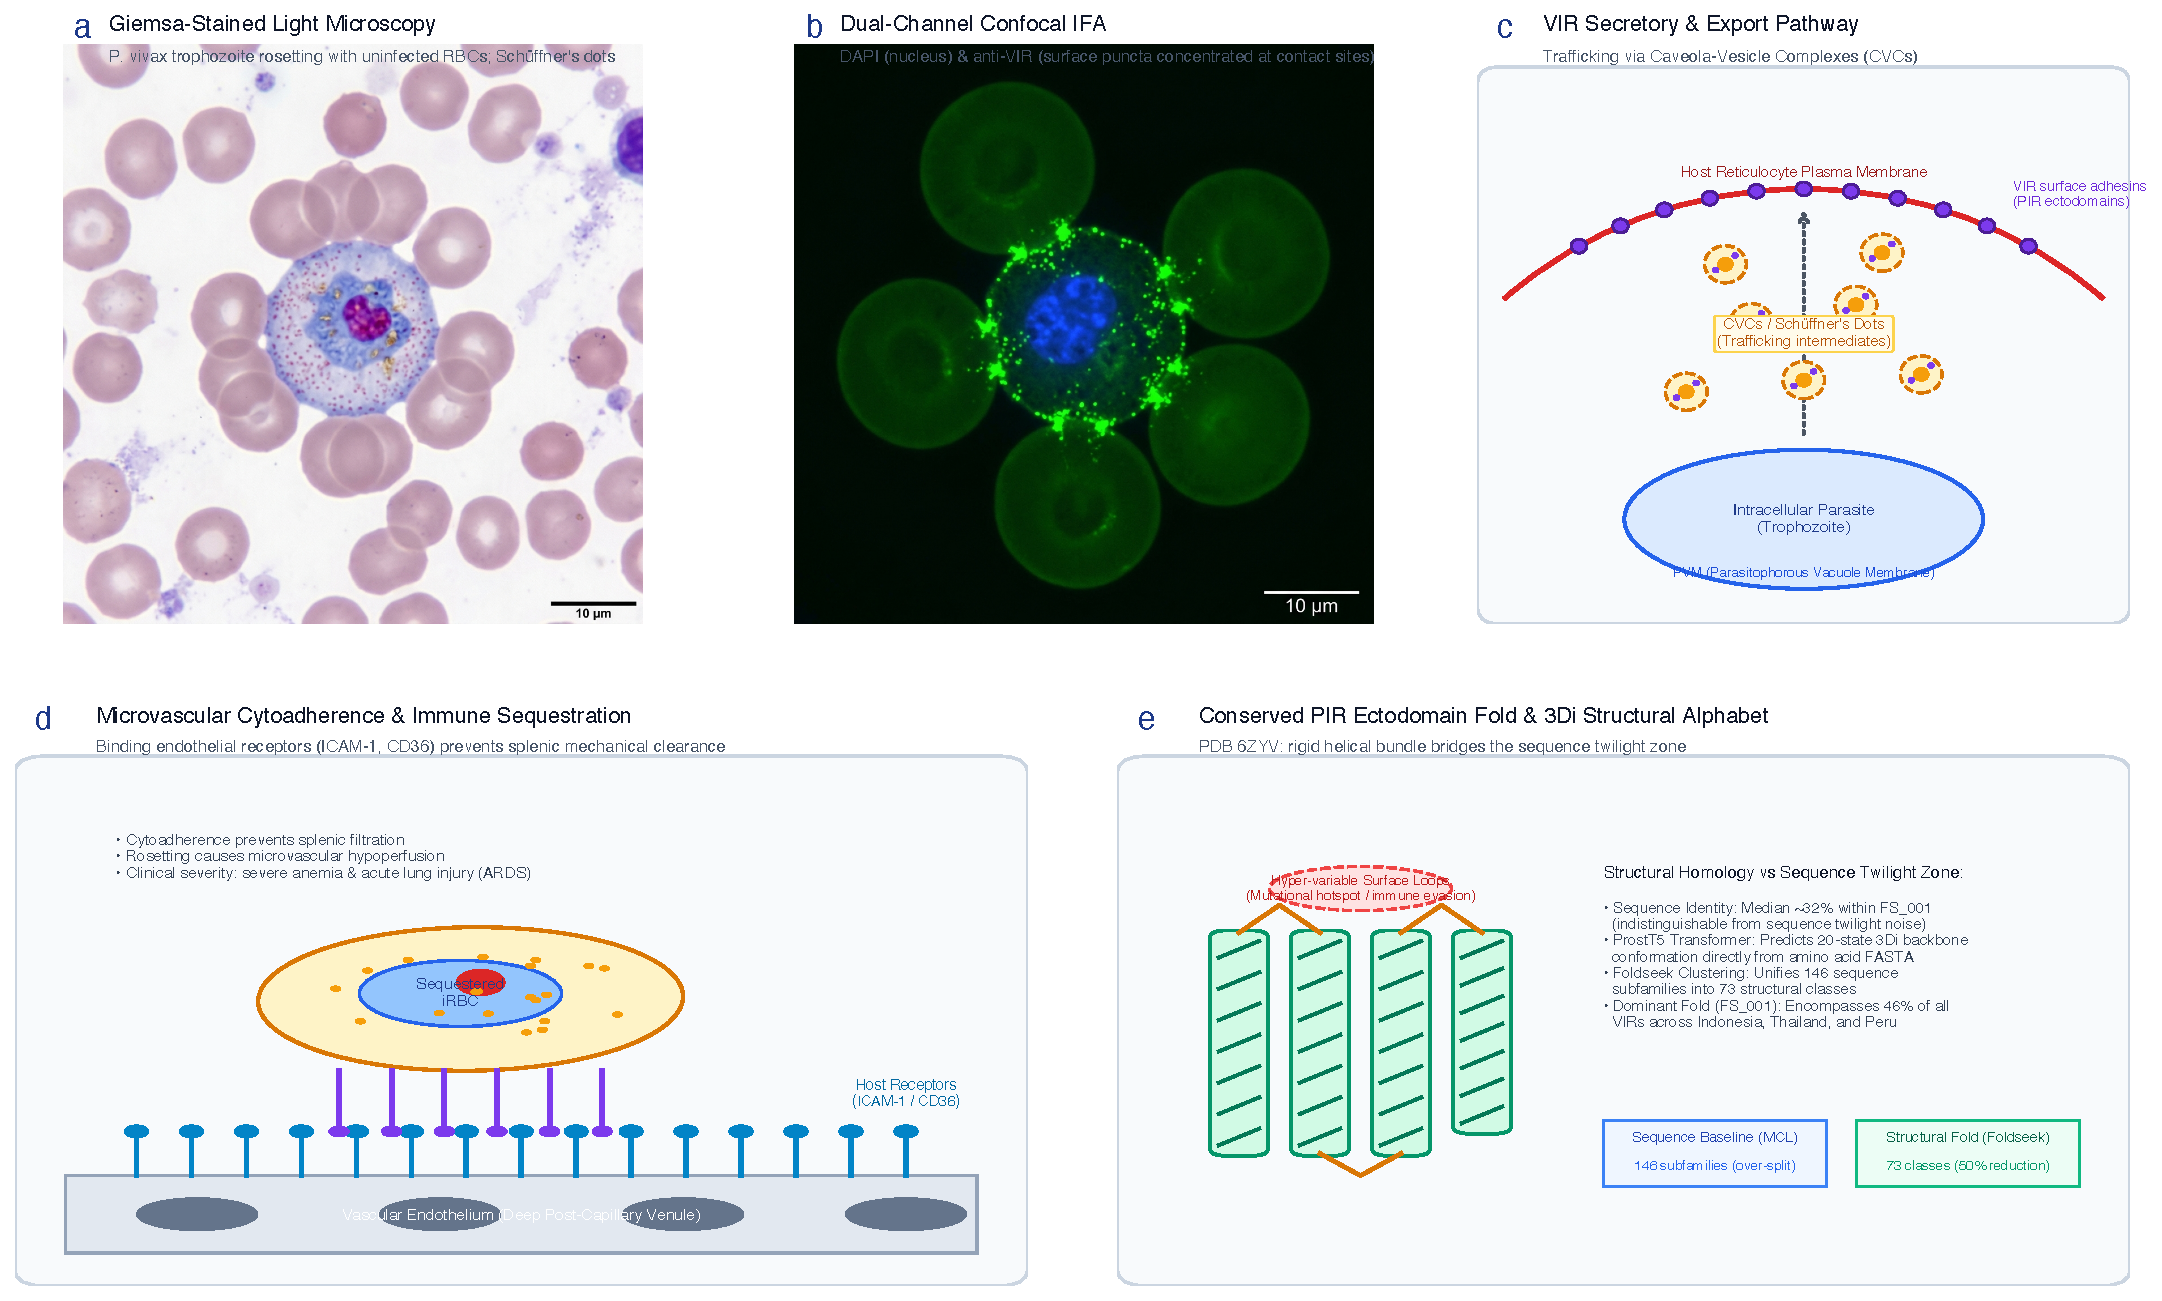
\includegraphics[width=\textwidth]{figures/figure2_pathogenesis_microscopy.pdf}
\caption{\textbf{Cellular pathogenesis, microscopy, rosetting, and conserved structural architecture of \textit{Plasmodium vivax} VIR surface antigens.} 
\textbf{a}, Brightfield light microscopy of a Giemsa-stained thin blood smear (100$\times$ oil immersion). An enlarged, polychromatophilic reticulocyte infected with an ameboid \textit{P. vivax} trophozoite forms a multicellular rosette with surrounding uninfected erythrocytes. Characteristic brick-red Schüffner's dots (stippling) pepper the host reticulocyte cytoplasm. Scale bar, 10\,$\mu$m. 
\textbf{b}, Dual-channel laser scanning confocal immunofluorescence microscopy (IFA). Parasite nucleus is stained with DAPI (blue). Exported VIR surface proteins are detected with anti-VIR antibodies conjugated to Alexa Fluor 488 (green), displaying punctate membrane localization concentrated at contact junctions with adhering uninfected red blood cells. Scale bar, 10\,$\mu$m. 
\textbf{c}, Secretory trafficking pathway. VIR proteins are synthesized by the intracellular trophozoite, cross the parasitophorous vacuole membrane (PVM), and travel through caveola-vesicle complexes (CVCs, corresponding to Schüffner's dots) to the host reticulocyte membrane. 
\textbf{d}, Deep microvascular cytoadherence. Infected reticulocytes adhere to host endothelial receptors (ICAM-1 and CD36) in post-capillary venules, escaping splenic filtration and triggering microvascular hypoperfusion. 
\textbf{e}, Conserved PIR ectodomain structural fold (PDB 6ZYV). A rigid four-helix bundle ($\alpha$1--$\alpha$4, green) provides structural stability, while hypervariable surface loops (red dashed outline) undergo rapid sequence diversification under humoral immune selection. Predicting 3Di structural alphabets directly from sequences with ProstT5 unifies 89 sequence subfamilies into structural class FS\_001.}
\label{fig:pathogenesis_rosetting}
\end{figure*}

\subsubsection*{Heavy-Weight User-Defined Tools and External Model Orchestration}
Executing this pipeline required computational capabilities completely absent from standard Tool Shed repositories. Modern structural phylogenomics operates over the structural 3Di alphabet rather than primary amino acids. To avoid the intractable computational cost of predicting three-dimensional coordinates for thousands of proteins, the pipeline predicts 3Di states directly from primary sequences using ProstT5. ProstT5 is a heavy deep-learning transformer model. Running ProstT5 requires 4.4 gigabytes of neural network weights (\texttt{prostt5-f16.gguf}), large memory allocations, and dedicated GPU acceleration.

Under standard agent frameworks, this requirement halts analysis. A local agent cannot install a 4.4-gigabyte foundation model on a consumer laptop without exhausting memory or colliding with host CUDA drivers. Commercial cloud runtimes demand private cluster configuration and substantial compute fees.

Our architecture resolved this limitation through unprivileged User-Defined Tools. The agent authored, registered, and executed ten distinct UDT definitions across twenty-seven revisions. To orchestrate heavy computational loads, the agent declared hardware resource requirements directly within the \texttt{GalaxyUserTool} definition:
\begin{center}
\small
\texttt{requirements: [\{type: resource, cores\_min: 32, ram\_min: 8192, cuda\_device\_count\_min: 1\}]}
\end{center}
Galaxy routed the job through naming conventions. Registering the tool identifier \texttt{anton-gpu-xl-\allowbreak foldseek\_prostt5\_clustering} directed the job to an NVIDIA A100-SXM4-40GB GPU node with CUDA 12.7 and thirty-two CPU cores. For CPU-bound tasks, the agent registered \texttt{anton-32-} tools, routing jobs to thirty-two-core compute nodes.

Container resolution presented severe operational hurdles. Initial attempts to run FoldMason failed because upstream containers lacked ProstT5 compilation flags. The agent diagnosed the defect through systematic hypothesis testing, isolating the root cause to the upstream binary. The agent resolved this impasse by implementing a purpose-built container (\nolinkurl{quay.io/nekrut/foldmason-prostt5:4.dd3c235-cpu}). To verify execution integrity, the agent instrumented UDTs to emit environment logs containing \texttt{nvidia-smi} diagnostics, CUDA driver versions, and allocated thread counts. Heavy foundational models executed remotely on public supercomputers without downloading neural weights or consuming local workstation memory.

\subsubsection*{Analytical Workflow Flowchart}
The investigation progressed through nine analytical modules spanning data ingestion, pseudogene rescue, structural clustering, microsynteny evaluation, and structural phylogenetics (Table~\ref{tab:phist_flowchart}).

\begin{table*}[htbp]
\centering
\small
\caption{\textbf{Analytical flowchart and execution ledger of the nine-step structure-aware phylogenomics pipeline.} Steps executed on UseGalaxy.org (History \texttt{bbd44e69cb8906b579031c61c5da0079}) through native tools and unprivileged User-Defined Tools.}
\label{tab:phist_flowchart}
\begin{tabularx}{\textwidth}{clp{4.2cm}p{3.8cm}X}
\toprule
\textbf{Step} & \textbf{Module} & \textbf{Tool \& UDT Wrapper} & \textbf{Compute Environment} & \textbf{Primary Data Transformation} \\
\midrule
1 & Ingestion & Native Galaxy Upload & Head node storage & Genomes, proteomes, GFF3s, and PF05795 profile loaded \\
2 & Functional Screen & \texttt{hmmer\_hmmsearch} (ToolShed) & Standard cluster slot & Profile HMM screen identifies 2,664 candidate VIR proteins \\
3 & Pseudogene Rescue & \texttt{gff\_pseudogene\_\allowbreak translator} (UDT) & 1 core (Python 3.12) & Six-frame translation of GFF3 pseudogenic transcripts \\
4 & Pseudogene Screen & \texttt{hmmer\_hmmsearch} (ToolShed) & Standard cluster slot & Rescues 75 PvP01 and 70 PvPAM pseudogenized VIR loci \\
5 & Structural Cluster & \texttt{foldseek\_prostt5} (UDT) & 32 cores + NVIDIA A100 & 4.4 GB ProstT5 model encodes 3Di; clusters 2,592 VIRs \\
6 & Structural MSA & \texttt{foldmason\_align} (UDT) & 32 cores (custom container) & Lockstep AA and 3Di structural alignment (10,128 columns) \\
7 & Microsynteny & \texttt{microsynteny\_\allowbreak filter} (UDT) & 8 cores (MMseqs2 + Python) & Filters 194 RBH pairs against 5,120 housekeeping backbone \\
8 & Spatial Profiling & \texttt{spatial\_analysis} (UDT) & 1 core (Python + SciPy) & Chromosomal coordinate mapping and label-shuffling tests \\
9 & Phylogenomics & \texttt{iqtree} (ToolShed) & 32 cores (multithreaded) & Partitioned ML tree inference (AA + 3Di substitution matrix) \\
\bottomrule
\end{tabularx}
\end{table*}

\subsubsection*{Summary of Empirical Results}
The structure-aware investigation yielded five decisive biological and methodological findings:

\begin{enumerate}
    \item \textbf{Structural clustering halves family complexity.} Conventional sequence clustering with MMseqs2 and Markov Clustering partitioned 2,592 VIR proteins into 146 sequence subfamilies. In contrast, Foldseek structural clustering collapsed the family into 73 structural classes. The dominant structural class, designated FS\_001, encompassed 1,197 proteins (46\% of the total repertoire) and merged 89 independent sequence subfamilies. Structural embeddings unified diversity that sequence comparisons over-split.
    \item \textbf{Universal structural conservation across continents.} Structural classes proved shared across geography. Over 97.3\% of all analyzed VIR proteins belonged to structural clusters containing members from Indonesia, Thailand, and Peru. Lineage-unique clusters accounted for only 2\% of sequences, consisting almost entirely of singletons. The structural scaffold of the VIR repertoire is globally conserved.
    \item \textbf{Absence of geographic phylogeographic signal.} Within the dominant FS\_001 cluster, we evaluated 338 sequence-subsampled representatives using maximum-likelihood structural phylogenetics (Fig.~\ref{fig:structural_phylogeny}a). Tip-label parsimony tests treating genome of origin as a discrete character yielded scores indistinguishable from random permutation ($p = 0.55$ for partitioned AA+3Di trees, $p = 0.69$ for AA alone, and $p = 0.26$ for 3Di alone, Fig.~\ref{fig:structural_phylogeny}b). Geographic lineages are interleaved across the tree. Diversification predated continental separation, and ongoing recombination maintains panmictic diversity.
    \item \textbf{Conserved subtelomeric architecture.} Coordinate analysis revealed that 64.5\% of chromosome-assigned VIR loci reside within the outer 10\% of chromosomal termini (Fig.~\ref{fig:genomic_organization}). Per-chromosome VIR counts correlated tightly across assemblies (Spearman $\rho = 0.909$ to $0.915$).
    \item \textbf{Sequence similarity generates false orthology.} Evaluating 194 reciprocal best-hit pairs between Thailand and Peru within FS\_001 revealed that only eleven pairs possessed conserved flanking microsynteny against the housekeeping backbone (Fig.~\ref{fig:synteny_twilight}). Sequence alignment alone misidentifies orthologs in dynamic multigene families.
\end{enumerate}

Every empirical claim was validated through automated verification scripts, passing seventy-seven independent assertions against raw outputs (77/77 PASS). By coupling autonomous agents to containerized User-Defined Tools and public supercomputers, our architecture executed an advanced structural phylogenomics pipeline without local hardware constraints or unrecorded computational steps.

\begin{figure*}[htbp]
\centering
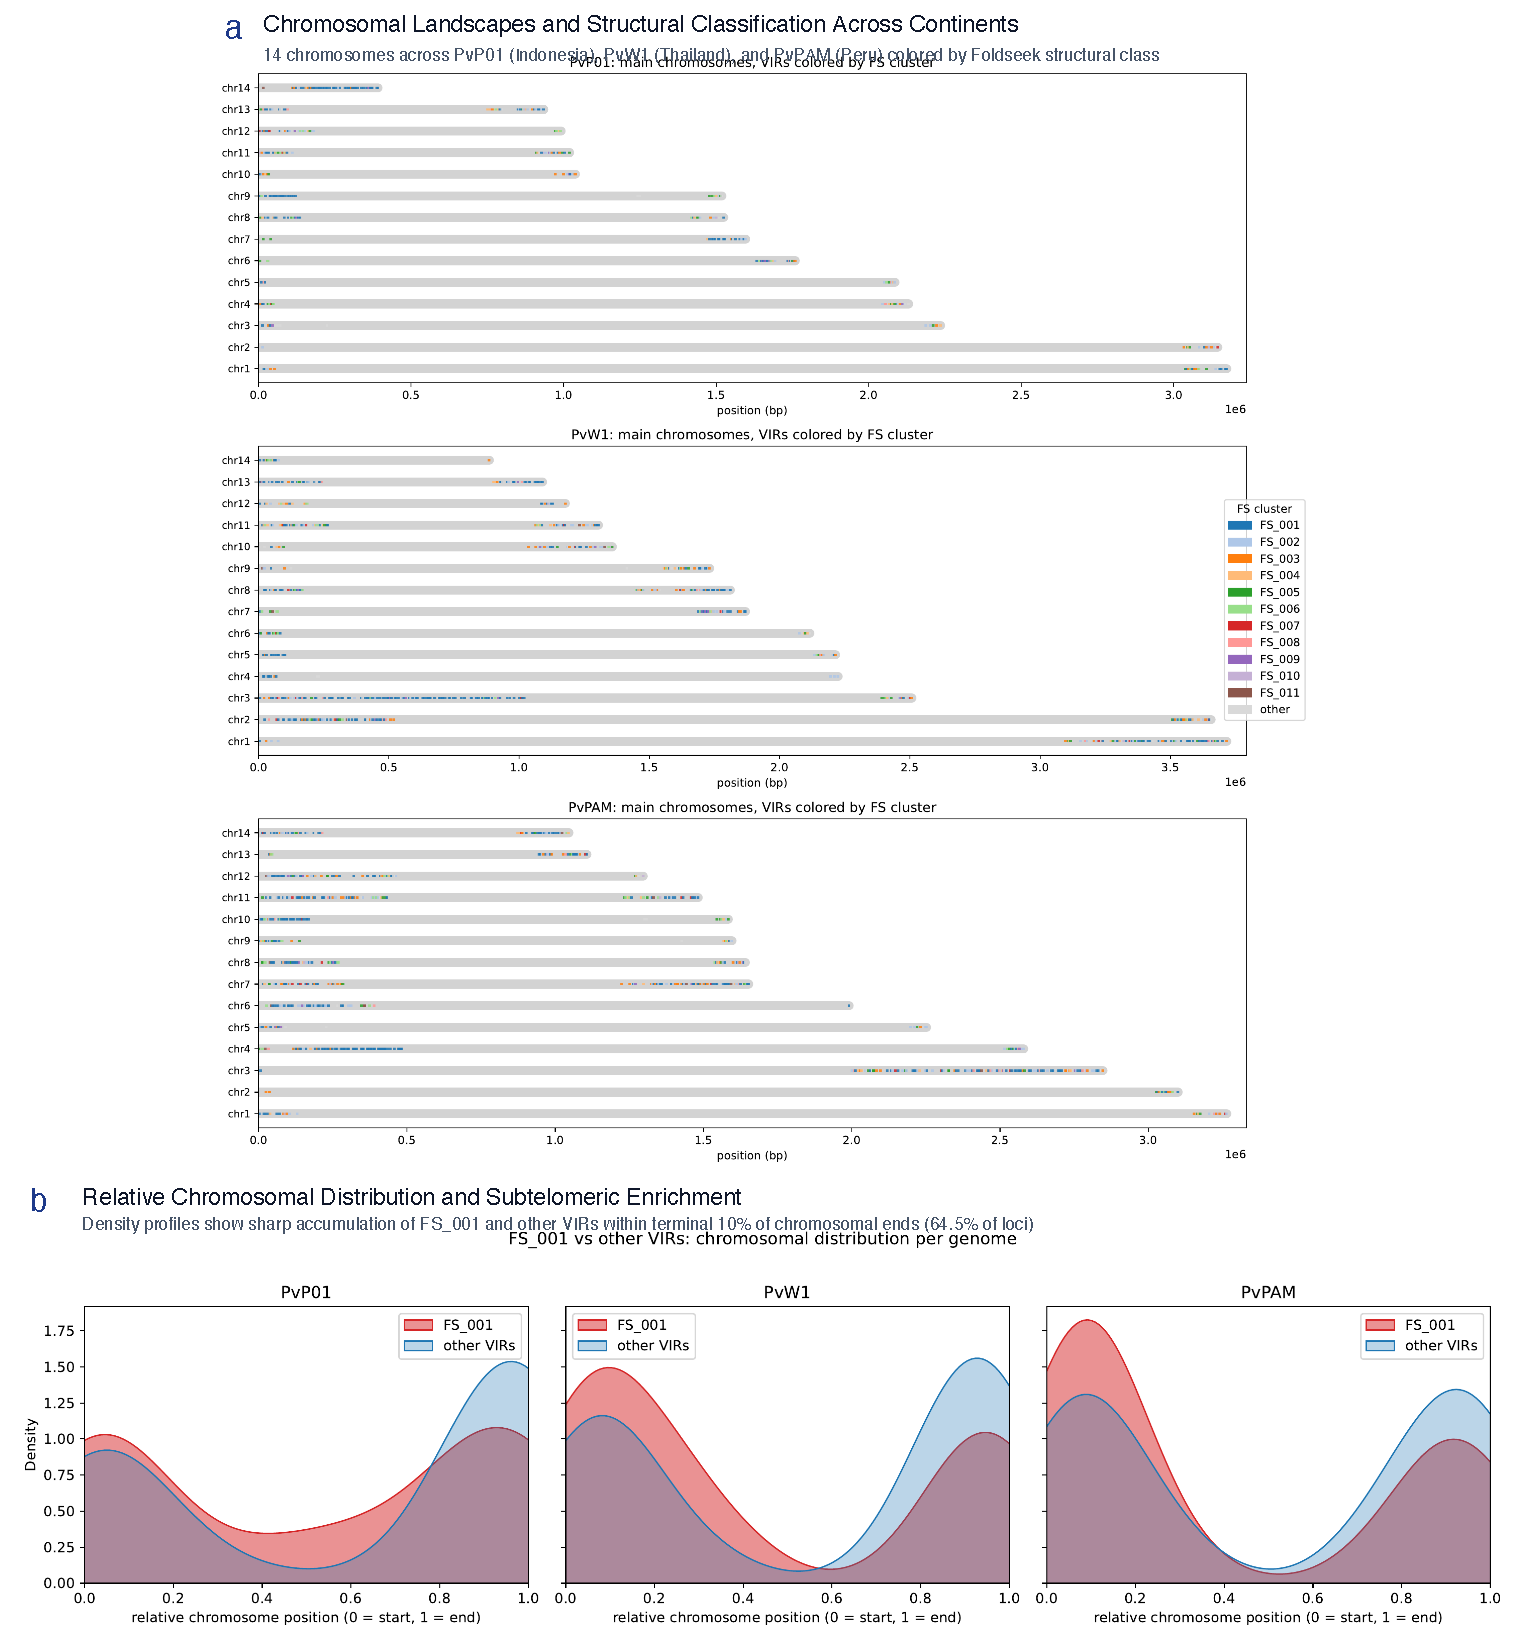
\includegraphics[width=\textwidth,height=0.66\textheight,keepaspectratio]{figures/figure3_genomic_organization.pdf}
\caption{\textbf{Chromosomal organization and subtelomeric compartmentalization of the VIR multigene family across continental assemblies.} 
\textbf{a}, Chromosomal ideograms for all fourteen nuclear chromosomes across three long-read assemblies: PvP01 (Indonesia), PvW1 (Thailand), and PvPAM (Peru). Each tick mark denotes a verified VIR locus, color-coded by its Foldseek structural class assignment. Structural clusters display conserved chromosomal footprints across continents. 
\textbf{b}, Relative chromosomal position density profiles comparing dominant structural class FS\_001 against all other VIR clusters. Terminal positions (0.0 and 1.0) represent chromosome ends. Both profiles show pronounced accumulation at chromosomal extremities, with 64.5\% of all loci residing within the terminal 10\% of chromosomes. Subtelomeric clustering acts as an evolutionary hotspot for ectopic recombination.}
\label{fig:genomic_organization}
\end{figure*}

\begin{figure*}[htbp]
\centering
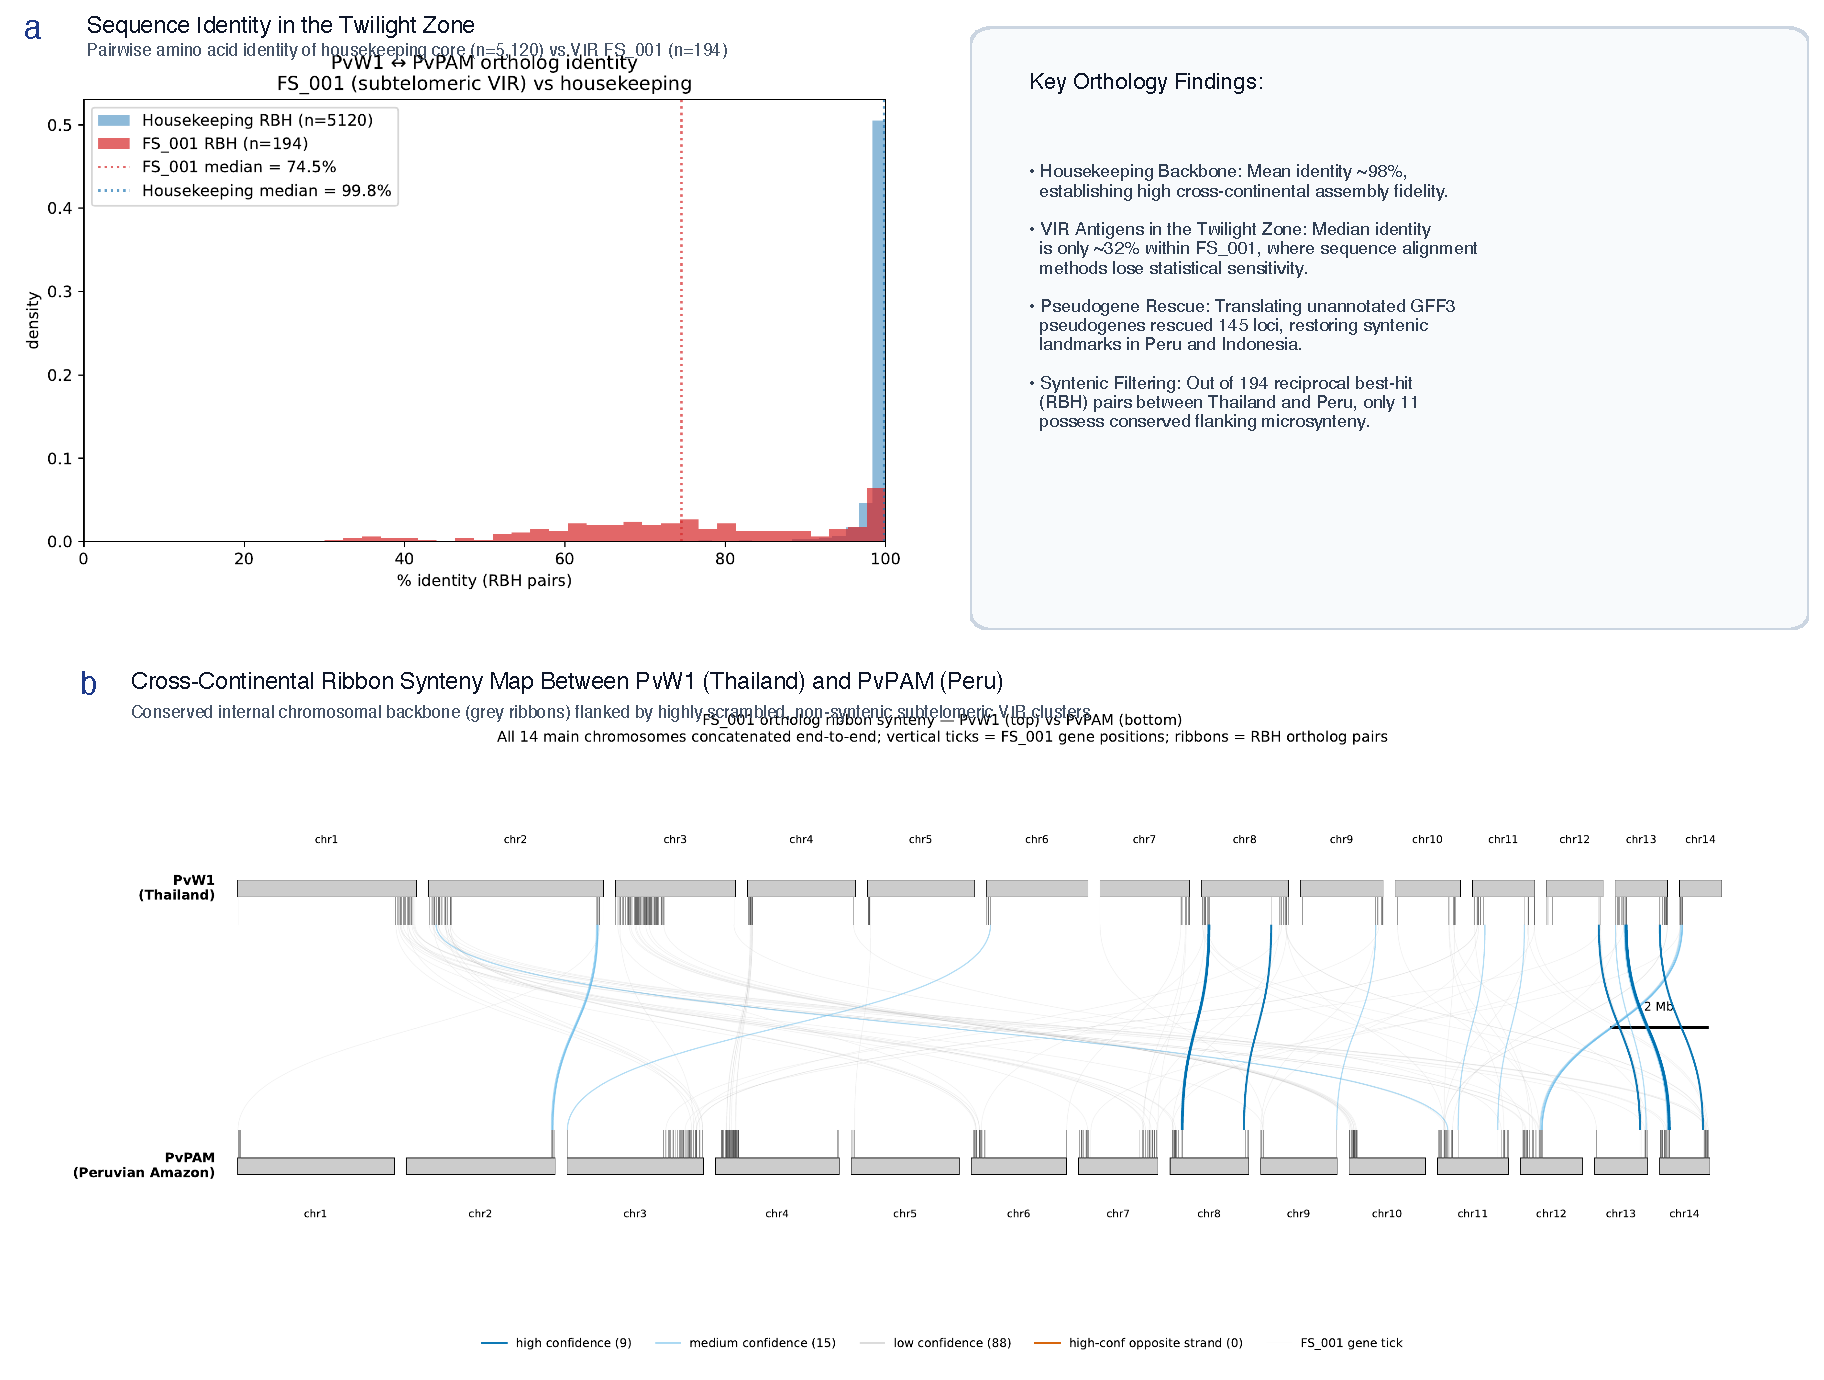
\includegraphics[width=\textwidth]{figures/figure4_synteny_twilight.pdf}
\caption{\textbf{The sequence twilight zone and breakdown of syntenic orthology in multigene antigen families.} 
\textbf{a}, Distribution of pairwise amino acid sequence identity between PvW1 (Thailand) and PvPAM (Peru). A reference backbone of 5,120 conserved core housekeeping genes exhibits high sequence identity (mean $\sim$98\%, blue), which confirms high assembly accuracy across continents. In contrast, 194 reciprocal best-hit pairs within the dominant VIR structural class FS\_001 exhibit a median sequence identity of only 32\% (red), residing squarely within the twilight zone where sequence alignment loses sensitivity. 
\textbf{b}, Whole-genome ribbon synteny map between PvW1 (top) and PvPAM (bottom). Grey ribbons denote conserved collinear syntenic blocks in the core chromosome backbone. Subtelomeric regions containing dense VIR clusters exhibit severe syntenic disruption and scrambling. Out of 194 reciprocal best-hit VIR pairs, only eleven maintain conserved flanking microsynteny against the housekeeping backbone.}
\label{fig:synteny_twilight}
\end{figure*}

\begin{figure*}[htbp]
\centering
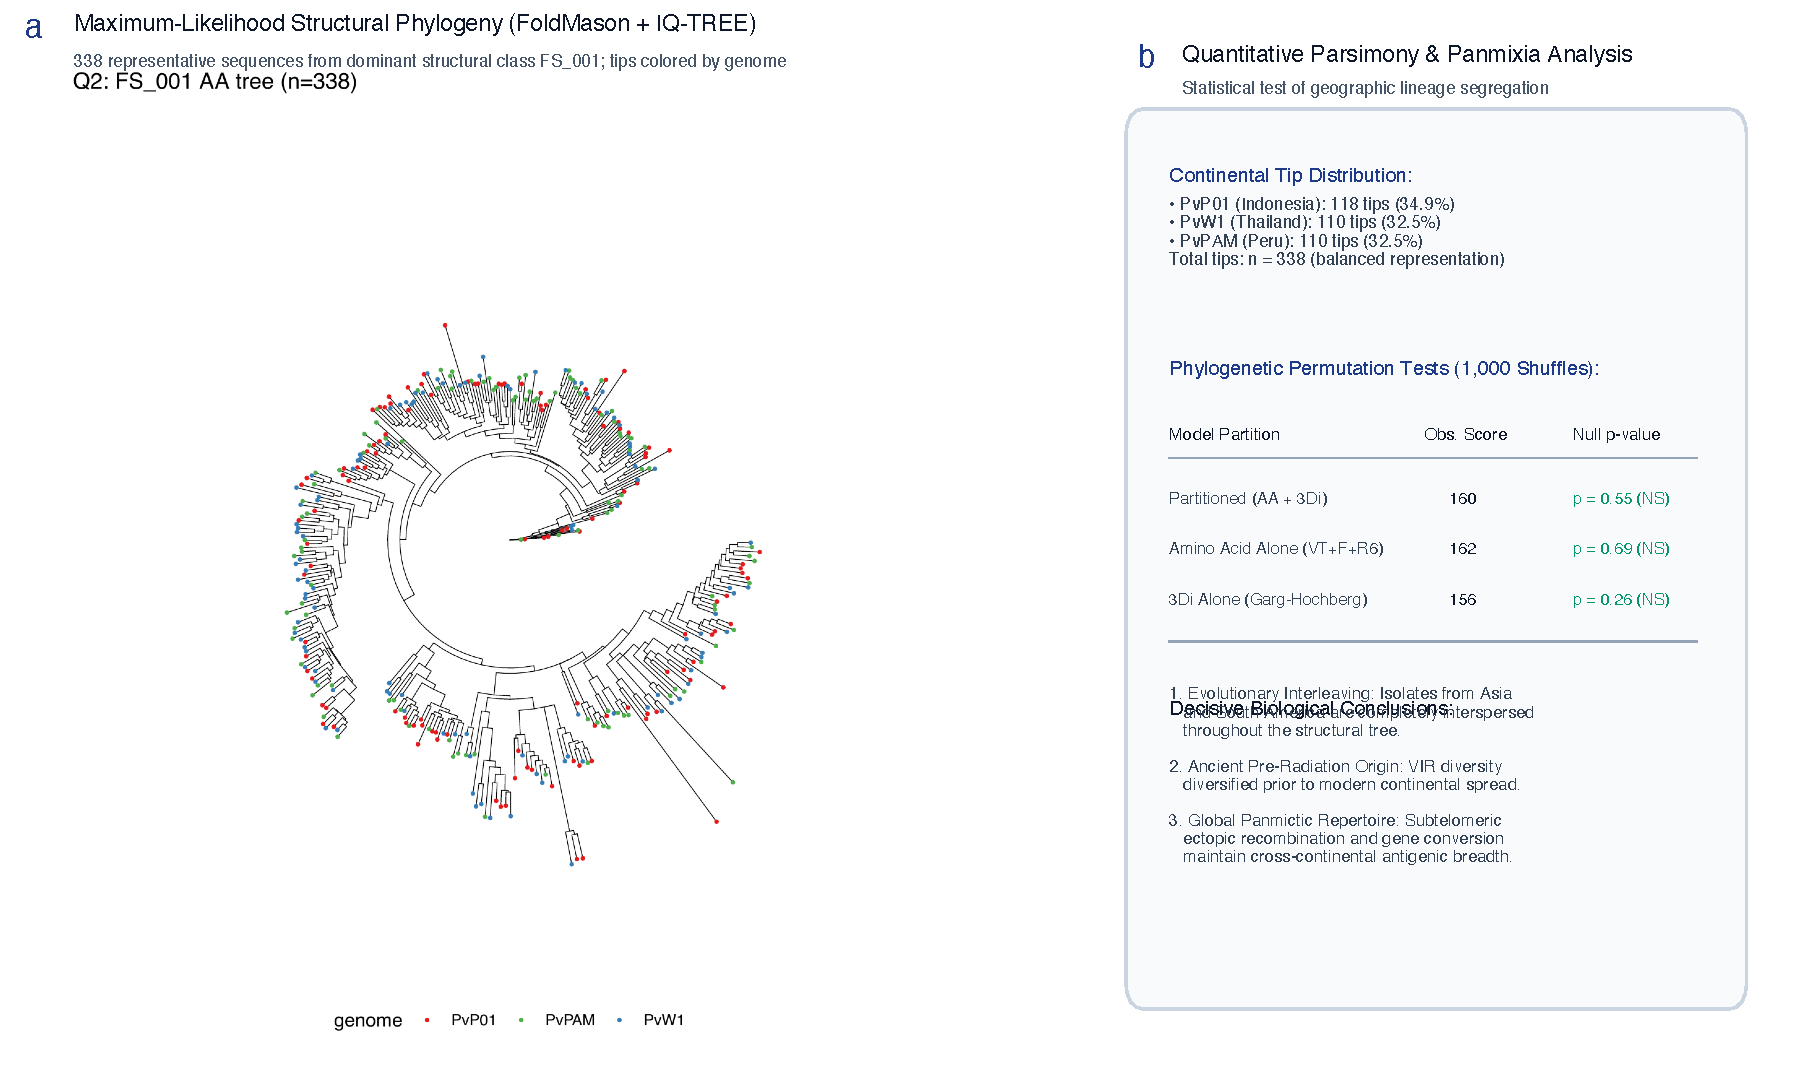
\includegraphics[width=\textwidth]{figures/figure5_structural_phylogeny.pdf}
\caption{\textbf{Global structural panmixia and phylogenomics of the dominant VIR fold across continents.} 
\textbf{a}, Circular maximum-likelihood structural phylogenetic tree inferred by IQ-TREE 3 from FoldMason multiple structural alignments of 338 sequence-subsampled representatives of dominant structural class FS\_001. The tree was inferred using partitioned models combining amino acid substitution matrices (VT+F+R6) and empirical 3Di structural alphabet matrices (Garg-Hochberg). Tip labels are color-coded by reference genome of origin: PvP01 (Indonesia, red), PvW1 (Thailand, green), and PvPAM (Peru, blue). Taxa from Southeast Asia and South America are thoroughly interleaved throughout the topology. 
\textbf{b}, Quantitative tip-label parsimony permutation tests. Observed parsimony scores of genome origin mapped onto the tree (score = 160 for partitioned AA+3Di, 162 for AA alone, and 156 for 3Di alone) do not differ significantly from 1,000 random tip permutations ($p = 0.55$, $p = 0.69$, and $p = 0.26$, respectively). This statistical independence demonstrates that VIR structural diversification preceded the continental divergence of modern \textit{P. vivax}, with ongoing subtelomeric recombination maintaining a panmictic global repertoire.}
\label{fig:structural_phylogeny}
\end{figure*}

\subsubsection*{Biological Summary: Structural Panmixia and Pathogenic Virulence}
The findings reshape our understanding of \textit{Plasmodium vivax} pathogenesis and antigenic evolution. Historically characterized as benign tertian malaria, \textit{P. vivax} causes severe clinical disease. Pathology includes acute respiratory distress syndrome, severe anemia, and placental malaria. These syndromes stem directly from the adhesive properties of VIR proteins exported to the host erythrocyte membrane (Fig.~\ref{fig:pathogenesis_rosetting}).

Unlike \textit{P. falciparum}, which infects erythrocytes across all developmental ages, \textit{P. vivax} restrictedly invades young reticulocytes expressing CD71. Following invasion, the ameboid trophozoite remodels the reticulocyte cytoplasm. The parasite establishes caveola-vesicle complexes that appear as classical Schüffner's dots under light microscopy (Fig.~\ref{fig:pathogenesis_rosetting}a). These membranous structures export VIR adhesins to the host erythrocyte surface (Fig.~\ref{fig:pathogenesis_rosetting}b,c). Once displayed on the membrane, VIR proteins mediate two distinct virulence phenotypes: endothelial cytoadherence and multicellular rosetting.

Rosetting occurs when an infected reticulocyte adheres to multiple uninfected erythrocytes. This interaction forms bulky multicellular clusters in peripheral circulation. These clusters obstruct post-capillary venules and cause microvascular hypoperfusion. Rosetting also shields the parasite from circulating antibodies. Concurrently, surface VIR adhesins bind endothelial receptors including ICAM-1 and CD36 (Fig.~\ref{fig:pathogenesis_rosetting}d). Cytoadherence enables infected cells to sequester in deep vascular beds and the spleen, escaping splenic clearance.

Immune evasion drives rapid mutation of external surface loops. This selective pressure plunges primary sequence identity into the twilight zone. Within the dominant structural class FS\_001, median pairwise sequence identity drops to 32\% (Fig.~\ref{fig:synteny_twilight}a). Sequence alignment tools interpret this divergence as evidence for independent gene families. Consequently, conventional Markov clustering fractures the repertoire into 146 subfamilies. Yet structural modeling reveals that these divergent sequences adopt a single conserved fold (Fig.~\ref{fig:pathogenesis_rosetting}e). The PIR ectodomain consists of a rigid, mostly-$\alpha$-helical bundle (PDB 6ZYV). By predicting 3Di structural alphabets directly from sequences with ProstT5, Foldseek unifies 89 sequence subfamilies into FS\_001, halving the apparent complexity of the repertoire.

This structural stability contrasts with extreme genomic instability. Coordinate mapping demonstrates that 64.5\% of VIR loci reside within the outer 10\% of chromosomal termini (Fig.~\ref{fig:genomic_organization}). While internal chromosomes maintain rigid colinear synteny across continents, subtelomeric domains are completely scrambled (Fig.~\ref{fig:synteny_twilight}b). Subtelomeric clusters act as an evolutionary recombination engine. High rates of ectopic exchange, unequal crossing over, and gene conversion reshuffle antigenic loops while preserving the core $\alpha$-helical chassis. Because recombination scrambles flanking genes, sequence similarity between continents produces false orthologs. Out of 194 reciprocal best-hit pairs between Thailand and Peru, only eleven maintain conserved flanking microsynteny.

The maximum-likelihood structural phylogeny resolves an enduring biogeographic debate (Fig.~\ref{fig:structural_phylogeny}a). Prior sequence analyses suggested that modern continental isolates underwent independent, lineage-specific expansions. Under this model, isolates from Indonesia, Thailand, and Peru should segregate into distinct clades. Instead, structural phylogenetics demonstrates complete evolutionary mixing. Taxa from South America and Southeast Asia interleave across the tree. Tip-label parsimony tests confirm that geographic distribution is indistinguishable from random permutation ($p = 0.55$, Fig.~\ref{fig:structural_phylogeny}b). Thus, the structural diversification of VIR antigens predated the continental radiation of modern \textit{P. vivax}. Ongoing subtelomeric recombination maintains a universally shared, panmictic antigenic reservoir across the globe.

\subsection{Case Study 2: Autonomous Translation of Published Papers into Workflows}
\begin{center}
\fbox{\parbox{0.9\textwidth}{\centering \textbf{[Case Study 2 Placeholder: Autonomous Literature Conversion]}\\[0.5em]
\small We evaluate autonomous workflow extraction directly from published scientific literature using the Workflow Foundry. The framework ingests methods sections and maps data flows to Tool Shed wrappers. When software is uncataloged, it synthesizes unprivileged User-Defined Tools. Continuous schema validation yields executable, community-standard \texttt{gxformat2} workflows.}}
\end{center}

\subsection{Case Study 3: Cross-Ecosystem Workflow Reusability}
\begin{center}
\fbox{\parbox{0.9\textwidth}{\centering \textbf{[Case Study 3 Placeholder: Nextflow to Galaxy Conversion]}\\[0.5em]
\small We demonstrate automated cross-ecosystem translation of complex pipelines from Nextflow DSL2 specifications into validated Galaxy workflows. The process maps containers to Bioconda packages, decomposes processes into verified Molds, and assembles test fixtures. This establishes functional equivalence across heterogeneous workflow engines.}}
\end{center}

\section{Discussion}

The integration of autonomous artificial intelligence into empirical science represents an epistemological turning point. If autonomous agents continue to operate as disembodied conversationalists inside private local environments, computational science will fragment into an unobservable collection of irreproducible, post-verifiable claims. By providing artificial intelligence with an open, distributed computational body, our architecture establishes a new paradigm: verifiable agentic science governed by provenance by construction.

\subsection{Provenance by Construction}
Scientific progress relies on the ability of independent researchers to inspect, challenge, and replicate computational findings. In conventional agent workflows, reproducibility depends entirely on post-hoc human discipline---an assumption that consistently fails in practice. Domain researchers interacting with conversational agents rarely record intermediate commands, pin operating system dependencies, or preserve raw data transformations.

Our architecture transfers the burden of reproducibility from human discipline to computational infrastructure. By executing analyses across Galaxy cyberinfrastructure, every analytical step is recorded upon an immutable directed acyclic graph. Tool versions, container digests, parameter values, and intermediate datasets are sealed in a permanent provenance ledger. This record is not an optional export---it is the physical mechanism through which compute occurs. Consequently, scientific claims generated through this framework carry complete execution lineage, ensuring that autonomous discoveries remain verifiable by the global scientific community.

\subsection{Democratizing the Scientific Commons}
The computational demands of frontier artificial intelligence threaten to centralize scientific discovery within well-funded commercial institutions. When automated research requires private compute clusters and proprietary cloud platforms, independent academic investigators are systematically excluded from high-throughput discovery.

We demonstrate that public, federally supported cyberinfrastructure can serve as the foundational execution surface for modern artificial intelligence. By pairing open foundation models and universal protocols with the Galaxy platform, we democratize autonomous science. A researcher at an under-resourced institution, equipped only with a standard laptop, can direct autonomous agents that orchestrate distributed supercomputing allocations, query petabyte-scale reference archives, and execute high-throughput pipelines across national high-performance clusters. Preserving the public scientific commons in the era of artificial intelligence is not merely an ethical priority---it is an infrastructural necessity for ensuring universal participation in scientific discovery.

\subsection{Toward a Verifiable Scientific Web}
Looking forward, coupling autonomous reasoning to open cyberinfrastructure establishes the foundation for a collaborative, planetary-scale scientific network. In this ecosystem, published workflows, curated reference databases, and execution engines communicate through standardized machine-readable protocols. Autonomous agents will not operate as isolated local assistants, but as distributed co-investigators capable of querying global workflow repositories, verifying analytical findings across independent compute clusters, and synthesizing collective biological knowledge. Grounding artificial intelligence in open, verifiable infrastructure ensures that the automated science of the coming decade remains transparent, reproducible, and universally accessible.

\section*{Methods}

\subsection*{Galaxy Model Context Protocol Implementation}
The Galaxy Model Context Protocol server (\texttt{galaxy-mcp}) is implemented in Python utilizing the official BioBlend library to communicate with the Galaxy REST API. The server supports two transport mechanisms: standard input-output (stdio) for local CLI integration and streamable HTTP for web and remote clients. Authentication occurs through long-lived Galaxy API keys or OAuth2 token exchanges. The server provides forty-four discrete tool functions mapped to Galaxy endpoints, implementing structured error handling and schema validation for all parameters.

\subsection*{User-Defined Tool Architecture}
User-Defined Tools are authored in YAML adhering to the \texttt{GalaxyUserTool} class definition. The tool wrapper specifies a mandatory container image hosted on public registries (Quay.io, Docker Hub), typed input parameters, declared output datasets, and an execution command. Commands are templated using sandboxed ECMAScript evaluation executed inside an isolated V8 runtime. Output files are claimed from the working directory through \texttt{from\_work\_dir} designations or dynamic dataset discovery patterns.

\subsection*{Orbit Workbench and Execution Guard}
Orbit is constructed as an Electron desktop application powered by a headless agent runtime built as an extension on Pi.dev. The runtime manages session context, system prompts, and tool registration. The execution guard intercepts tool calls via internal lifecycle hooks, classifying actions across model tiers, path security, and shell hazard. Local file writes are strictly confined to the workspace root using realpath resolution. Remote Galaxy jobs are tracked through YAML invocation blocks embedded within \texttt{notebook.md}, which are updated via background polling and asynchronous event handlers.

\subsection*{Workflow Foundry Casting Pipeline}
The Workflow Foundry compiler is implemented in TypeScript and Node.js. Molds are authored as Markdown documents carrying structured Zod-validated YAML frontmatter declaring pattern dependencies, manual references, and input-output schemas. The casting pipeline compiles Molds into target-specific agent skills. Synthesized workflows are validated statically using the \texttt{gxwf} validation engine, which verifies graph topology, step connectivity, and tool state against official Galaxy XML schemas and IWC exemplars.

\section*{Data and Code Availability}
All software components developed in this work are open-source and publicly available:
\begin{itemize}
    \item Galaxy MCP Server: \url{https://github.com/galaxyproject/galaxy-mcp}
    \item Orbit Workbench and Loom Runtime: \url{https://github.com/galaxyproject/loom}
    \item Workflow Foundry: \url{https://github.com/galaxyproject/foundry}
    \item Galaxy Skills and Developer Guides: \url{https://github.com/galaxyproject/galaxy-skills}
    \item Universal Agentic Plugins: \url{https://github.com/galaxyproject/agentic-plugins}
\end{itemize}
All case study datasets, analysis notebooks, and Galaxy history records are accessible via the project repository: \url{https://github.com/galaxyproject/orbit-paper}.

\bibliographystyle{plain}
\bibliography{references}

\end{document}
